\section{Desarrollo de juegos serios}
\label{sec:desarrollo}

Una vez definido lo que es un juego serio, queda la tarea de definir cómo
realizar uno, incluyendo qué factores deben ser tomados en cuenta durante su desarrollo.
% Esto hacemos/ esto de los problema comunes? wtf no me acuerdo de haber leido nunca esto

Según~\cite{education:games} un juego serio debe cumplir los siguientes
tres criterios:

\begin{itemize}

\item \textbf{Implementación técnica}: se refiere a la actividad de programación
    y ejecución de un patrón de diseño. Incluye la perfecta integración de los
    elementos de diseño en el videojuego. 

\item \textbf{Adecuación para la educación:} la capacidad del videojuego para hacer
    frente a las metas curriculares o educativas y la habilidad o el
    conocimiento del jugador relativo a los contenidos educativos que se aborde.

\item \textbf{Integración total con los objetivos pedagógicos:} la integración
    del patrón de diseño y el videojuego en general con los objetivos
    educativos.

\end{itemize}


Adicionalmente, el diseño del mismo se tiene que centrar en cuatro factores o
dimensiones, las cuales son\cite{education:games}:

\begin{itemize}
\item \textbf{Contexto:} es decir, donde ocurre el aprendizaje, lo que va desde
    aspectos macro, como  factores políticos, económicos e históricos, hasta
    aspectos micro como la experiencia y  antecedentes de los profesores, costos
    de licencia, entre otros.
\item \textbf{Tipo de aprendizaje:} para el individuo o grupo, requiere que se
    considere su  estilo de aprendizaje y sus conocimientos previos, y qué
    métodos se ajustan mejor a sus  necesidades.
\item \textbf{Modo de representación:} lo que incluye el nivel de interactividad
    requerido, la fidelidad y  el nivel de inmersión producido. Además cubre la
    narración de los hechos, la separación de los  aspectos de inmersión con la
    reflexión de haber utilizado el videojuego. Y de manera importante  enfatiza
    el potencial de retroalimentación que refuerza el aprendizaje.
\item \textbf{Principios pedagógicos:} es necesario reflexionar sobre los
    modelos de aprendizaje lo  que permite producir apropiados planes de
    lecciones.
\end{itemize}

Estas dimensiones no pueden ser consideradas individualmente, todas están
relacionadas  como se muestra en el figura~\ref{fig:desarrollo_dimensiones}.

\begin{figure}[H]
\centering
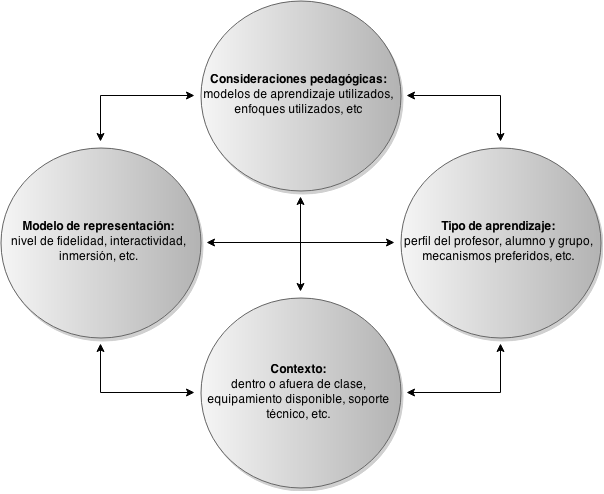
\includegraphics[scale=0.5]{juegos_serios/desarrollo_dimensiones.png}
\caption{Relación entre las cuatro dimensiones a considerarse en un videojuego
    basado en aprendizaje}
\label{fig:desarrollo_dimensiones}
\end{figure}

A continuación se da un ejemplo de flujo de diseño para implementar un juego serio 
manteniendo todas sus características incluyendo los criterios y factores descritos 
anteriormente.

\subsection{Flujo de diseño de un juego serio}

\textit{Pereira}\cite{pereira2009design} en el diseño del videojuego \emph{Living
    Forest} utiliza un conjunto de pasos bien definidos como modelo de creación
de un juego serio a partir de la definición previa de las competencias básicas
que se desean enseñar.

Es importante notar que este modelo se adecua a las dimensiones y criterios
definidos previamente. La obtención de las competencias básicas no forma parte
de este flujo pues, se asume que es un paso previo al diseño.

\begin{figure}[ht!]
\centering
\begin{tikzpicture}[auto]
    % Place nodes
    \node [block] (1) {1. Objetivos de diseño};
    \node [block, right of=1, node distance=5cm] (2) {2. Competencias básicas relacionadas con la educación};
    \node [block, right of=2, node distance=5cm] (3) {3. Investigación del dominio};
    \node [block, below of=3, node distance=3cm] (4) {4. Diseño del juego};
    \node [block, left of=4, node distance=5cm] (5) {5. Tiempo en el juego};
    \node [block, left of=5, node distance=5cm] (6) {6. Acciones de jugabilidad};
    \node [block, below of=6, node distance=3cm] (7) {7. Indicadores};
    \node [block, right of=7, node distance=5cm] (8) {8. Representación e interacción};
    \node [block, right of=8, node distance=5cm] (9) {9. Implementación};
    \node [block, below of=9, node distance=3cm] (10) {10. Evaluación};
    % Draw edges
    \path [line] (1) -- (2);
    \path [line] (2) -- (3);
    \path [line] (3) -- (4);
    \path [line] (4) -- (5);
    \path [line] (5) -- (6);
    \path [line] (6) -- (7);
    \path [line] (7) -- (8);
    \path [line] (8) -- (9);
    \path [line] (9) -- (10);
\end{tikzpicture}
\caption{Flujo de diseño propuesto de un juego serio}
\label{fig:tics_flujo_diseño_prop}
\end{figure}

Teniendo las competencias básicas que se desea sean enseñadas, practicadas o
perfeccionadas por el usuario mientras utiliza el juego serio a diseñar, los
siguientes puntos que deben ser diseñados son
(ver~\ref{fig:tics_flujo_diseño_prop}):

\begin{enumerate}
\item \textbf{Objetivos de diseño:} definen cuál es el propósito del videojuego, donde
    se toman en cuenta los objetivos pedagógicos, así como también objetivos que
    garanticen que el mismo sea agradable, intuitivo y motivador.

\item \textbf{Competencias básicas relacionadas con la educación:} se identifican
    aquellas que influyen en el diseño del videojuego, se definen los conocimientos
    mínimos que se desea que tenga un usuario que lo utilice.

Las competencias básicas pueden tener diferentes orígenes, en el ámbito
académico se puede utilizar el plan de estudios, en una empresa se pueden
utilizar los objetivos y la visión de la misma.

\item \textbf{Investigación del dominio:} esta fase se encarga de recabar
    información exacta acerca del dominio en el cual se desenvuelve el juego
    serio, en esta fase es importante que participe un experto en el dominio,
    por ejemplo, en el ámbito académico se puede contar con un profesor experto
    en el dominio.

Es importante realizar la pregunta \emph{¿Qué nivel de detalle es necesario?},
para así definir qué contenido incluir, y qué factores se deben analizar.

Además es necesario investigar las acciones que se podrían realizar dentro del
videojuego, cómo se desenvolverá el jugador, por cada acción definida, se deben
analizar los elementos y factores relacionados que se deben modelar.

\item \textbf{Diseño del juego:} a partir de la idea original y basado en la
    información recogida se determina el papel desempeñado por el jugador (de
    acuerdo a la semántica y pragmática de las acciones y decisiones que está
    llamado a hacer). 

Se define el nivel de aproximación a la realidad, el nivel de detalle del
entorno, del jugador y de las acciones.

Otro factor que se debe tener en cuenta en esta fase es la cantidad de tiempo
que pasará un jugador en el juego, se deben modelar todas las acciones del
jugador y el entorno de acuerdo a este tiempo.

\item \textbf{Tiempo de juego:} el primer factor que se debe estudiar es el
    período de adaptación del jugador, lo que depende de la intuitividad del
    videojuego, este tiempo debe ser analizado por separado a la hora de realizar un
    análisis de los resultados.
    
    Se debe definir la duración de las partidas y la forma en la que 
    se mostrarán los resultados de las acciones.
% Esto es jodido por que no hicimos, osea mmm no se
%Si el videojuego tiene una duración reducida, se tienen que analizar mecanismos %para
%mostrar los resultados de las decisiones a largo plazo, además de como mostrar
%los resultados de las acciones de corto plazo.

\item \textbf{Indicadores:} es todo aquello que muestre información relevante al
    jugador acerca de su estado, ejemplos de este tipo de indicadores son el
    puntaje, tiempo empleado, objetivos cumplidos. 

La definición de como se juzgará la calidad de una partida del jugador debe ser
definida, normalmente mediante un puntaje general, el mismo debe mostrar
claramente los resultados de las acciones, si las mismas fueron positivas o
negativas para el logro final de los objetivos.

\item \textbf{Representación e interacción:} representación se refiere a como se
    visualiza el entorno, e interacción a como se relaciona el jugador con su
    entorno.

Se inicia con un bosquejo de las representaciones de la escena del videojuego, para
así poder definir los elementos que forman parte de la escena.

Otros bosquejos necesarios son los del concepto que se modela en la lógica del
videojuego, para así definir las animaciones del entorno y del jugador.

Se deben definir las alertas sonaras, qué partes del entorno produce sonidos,
cómo el jugador recibe estas alertas (por ejemplo si el origen de las mismas es
siempre el mismo o importa la distancia a la cámara), se puede agregar música de
ambiente si el videojuego lo amerita.

Se define la interfaz del usuario, qué información será representada, las
acciones disponibles desde la misma, además se define si el mismo será en
primera persona (la cámara son los ojos del jugador) o en tercera persona (la
cámara se sitúa inmediatamente atrás y arriba de la cabeza), como será la
interacción con la cámara, acercamientos y movimientos para contemplar el
entorno.

\item \textbf{Implementación:} en esta etapa se estudia el estado del arte de las
    plataformas tecnológicas disponibles para el desarrollo del videojuego, se toman
    en cuenta los factores como la disponibilidad de componentes, de
    documentación, lenguajes de programación y herramientas de pruebas
    automáticas.

El proceso puede ser iterativo, entre sesiones de implementación y evaluación de
lo implementado, para así poder realizar optimizaciones enfocadas especialmente
en la estética, la retroalimentación y el estado del jugador.

\item \textbf{Evaluación:} durante el desarrollo del juego serio, se deben
    realizar varias sesiones de evaluación, por ejemplo, con los responsables o
    expertos y miembros de la audiencia objetivo. Así mismo, se deben realizar
    evaluaciones con los grupos de interés las cuales se centran en la adaptación
    del videojuego (usabilidad). 

La primera evaluación mencionada se centra en la validación del modelo de la simulación
(refinamiento), mientras que la segunda evaluación sirve para probar el videojuego en
un escenario (parecido al final) y evaluar los aspectos relacionados con el
proceso de aprendizaje.  

\end{enumerate}
